\documentclass[12pt]{article}
\usepackage{geometry}
\usepackage{dcolumn}
\usepackage{booktabs}
\usepackage{pdflscape}
\usepackage{graphicx}
\usepackage{placeins}
\usepackage{dcolumn}
\usepackage{xcolor}
\usepackage{booktabs}
\linespread{1.5}
\usepackage{subcaption}
\usepackage{amsmath}
\usepackage{hyperref}
\usepackage{multirow}
\usepackage[title]{appendix}
%\usepackage{xepersian}
%\settextfont{XB Zar}
%\setdigitfont{XB Zar}


\renewcommand{\today}{\ifcase \month \or January\or February\or March\or %
April\or May \or June\or July\or August\or September\or October\or November\or %
December\fi, \number \year} 

\begin{document}
\nopagebreak
\newgeometry{margin = 1.2cm}
\title{
 Capital Raise and Price Impact \\
  \large 
 Impact of capital raise on return of firms 
  }
\author{S.Morteza Aghajanadeh}

\nopagebreak
{\maketitle}

Data contains a $ 3721 $  capital rise for $ 800 $ firms in Tehran Stock Exchange. Some of these events have happened before IPO, which may not impact the stock price. 
We have three different sources for capital rising: Cash, Saving, and premium. Table   \ref{t1} may demonstrate each source's share from the mentioned sources in capital raising.

\begin{table}[htbp]
  \centering
  \caption{Different sources for Capital raise in Data}
\label{t1}
\begin{tabular}{l|cccc}
          & \multicolumn{1}{l}{Cash} & \multicolumn{1}{l}{Saving} & \multicolumn{1}{l}{Premium} & \multicolumn{1}{l}{Hybrid} \\
          \hline
    Event  & 2217 & 1056 & 103 & 344 \\
     Percent  & 59.61\% & 28.38\% & 2.77\% & 9.24\% 
    \end{tabular}%
  \label{tab:addlabel}%
\end{table}%






\begin{figure}
\centering
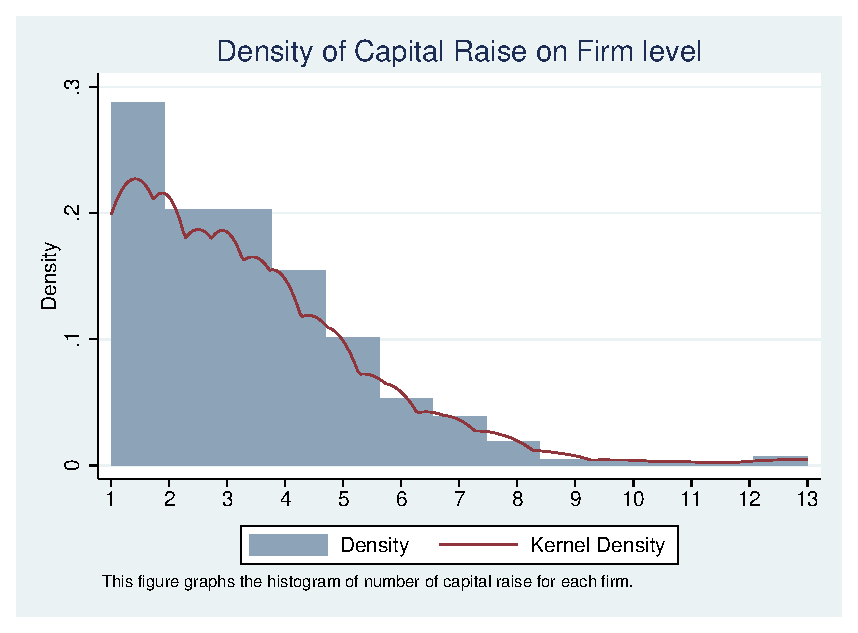
\includegraphics[width=0.7\linewidth]{Hist.eps}
\caption{}
\label{fig:Hist}
\end{figure}

\begin{figure}
\centering
\includegraphics[width=0.7\linewidth]{MedianCapRaise.eps}
\caption{}
\label{fig:mediancapraise}
\end{figure}

\begin{figure}
\centering
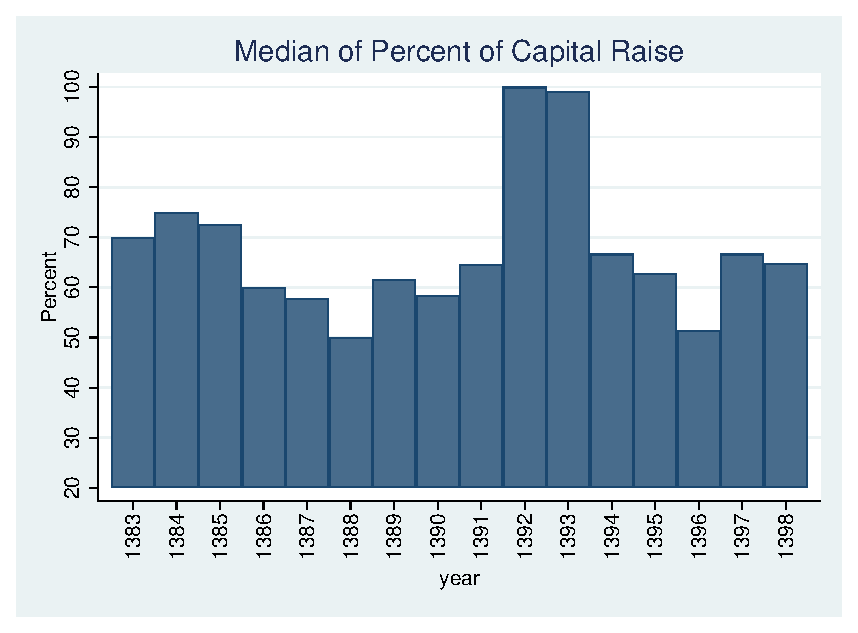
\includegraphics[width=0.7\linewidth]{MedianPercent.eps}
\caption{}
\label{fig:medianpercent}
\end{figure}

\begin{figure}
\centering
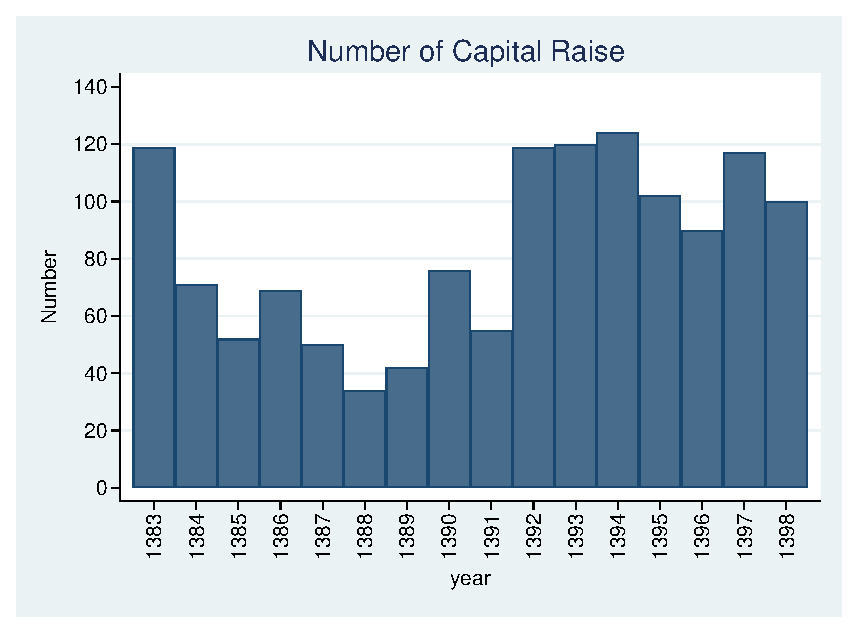
\includegraphics[width=0.7\linewidth]{Number.eps}
\caption{}
\label{fig:number}
\end{figure}

\begin{figure}
\centering
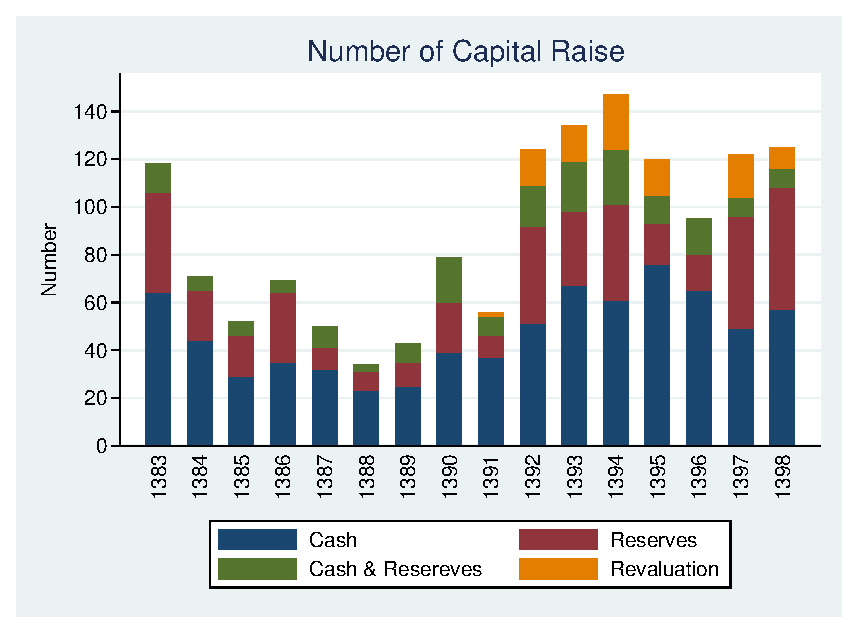
\includegraphics[width=0.7\linewidth]{Number2.eps}
\caption{}
\label{fig:number2}
\end{figure}

\begin{figure}
\centering
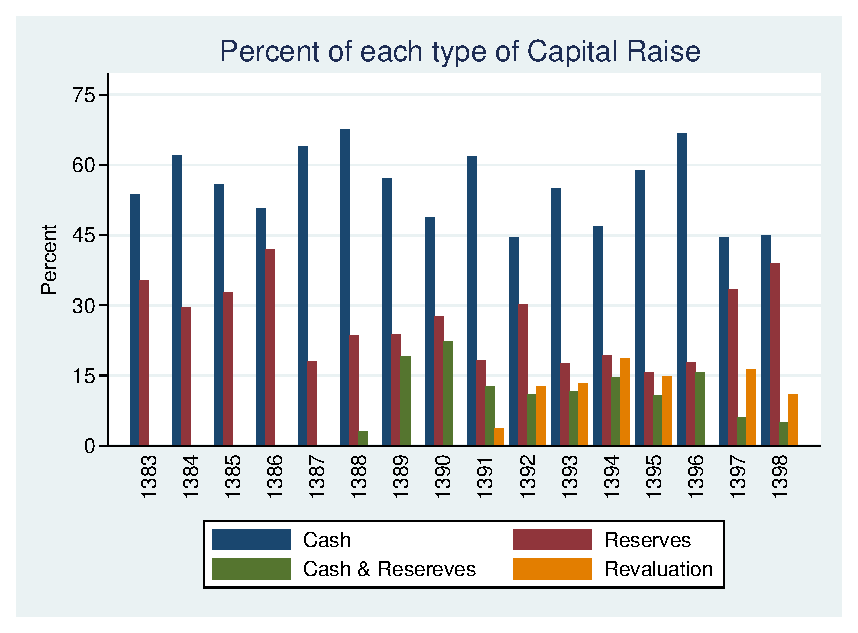
\includegraphics[width=0.7\linewidth]{Number3.eps}
\caption{}
\label{fig:number3}
\end{figure}

\begin{figure}
\centering
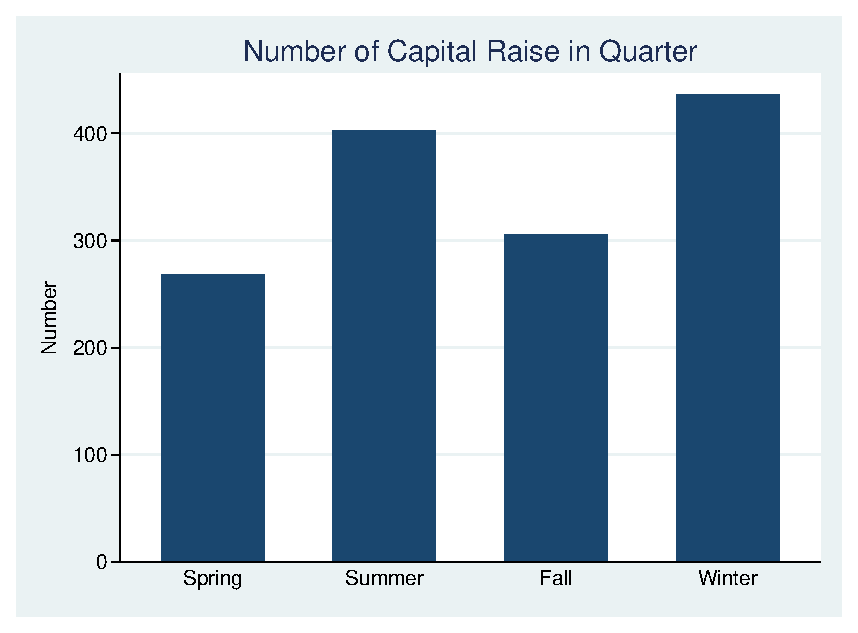
\includegraphics[width=0.7\linewidth]{QNumber}
\caption{}
\label{fig:qnumber}
\end{figure}

\begin{figure}
\centering
\includegraphics[width=0.7\linewidth]{QNumber2}
\caption{}
\label{fig:qnumber2}
\end{figure}


\begin{figure}
\centering
\includegraphics[width=0.7\linewidth]{QNumber3}
\caption{}
\label{fig:qnumber3}
\end{figure}






\begin{landscape}
\begin{figure}
\centering
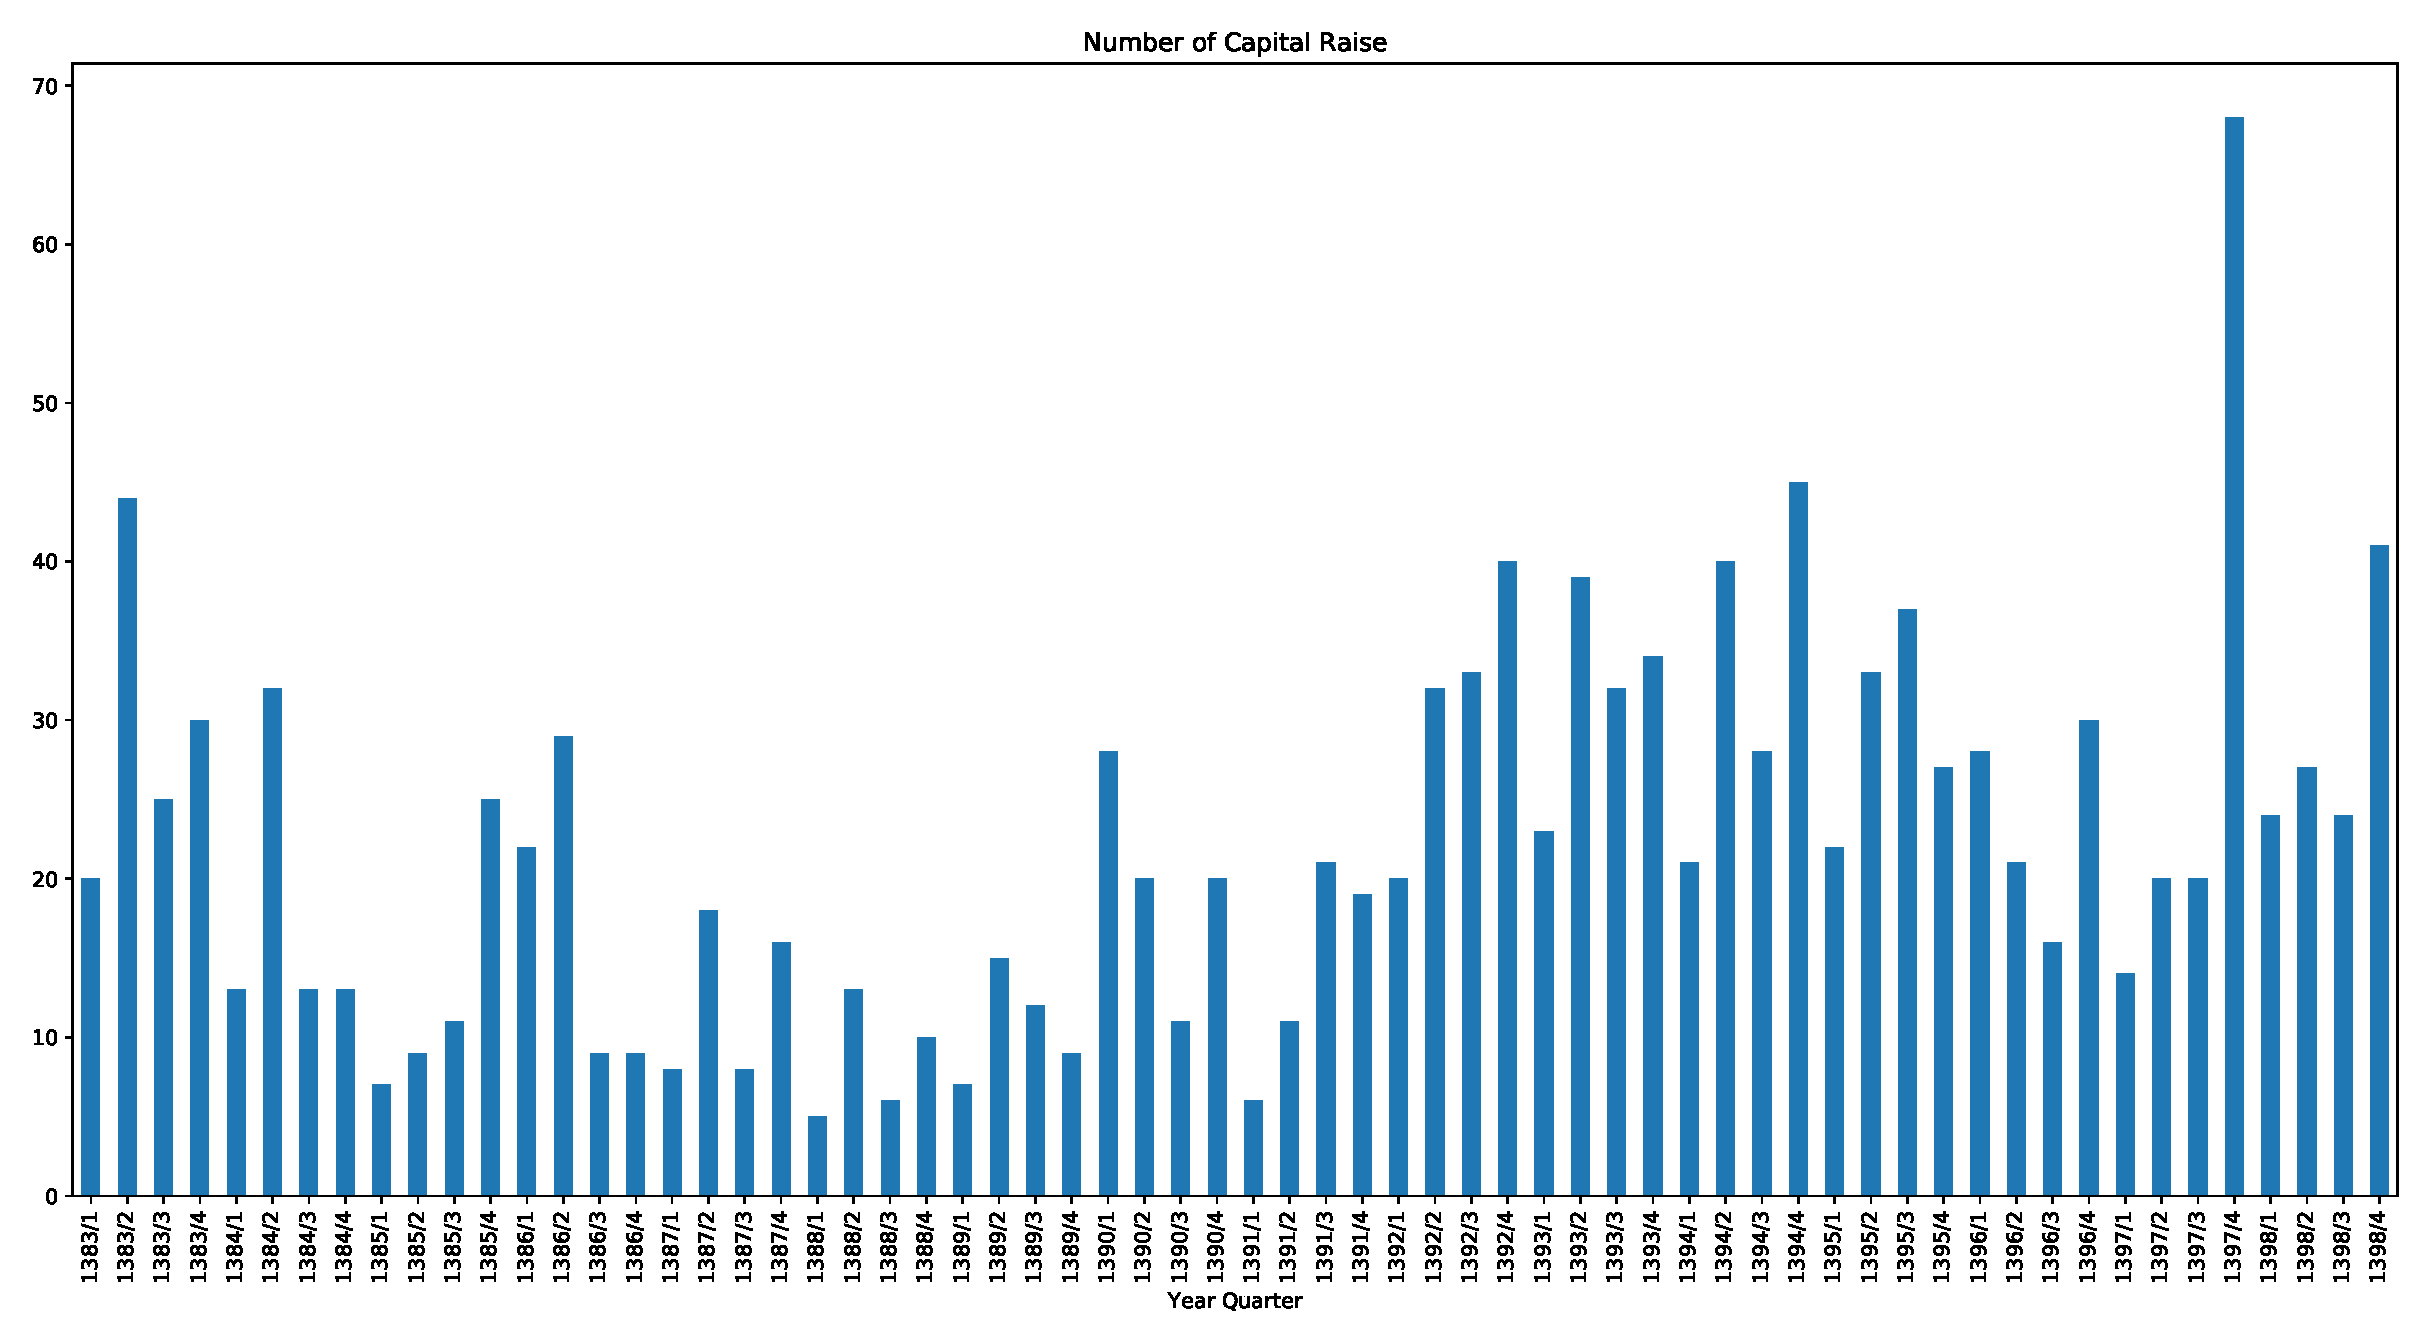
\includegraphics[width=1\linewidth]{Q2Number}
\caption{}
\label{fig:q2number}
\end{figure}
\end{landscape}
\begin{landscape}
\begin{figure}
\centering
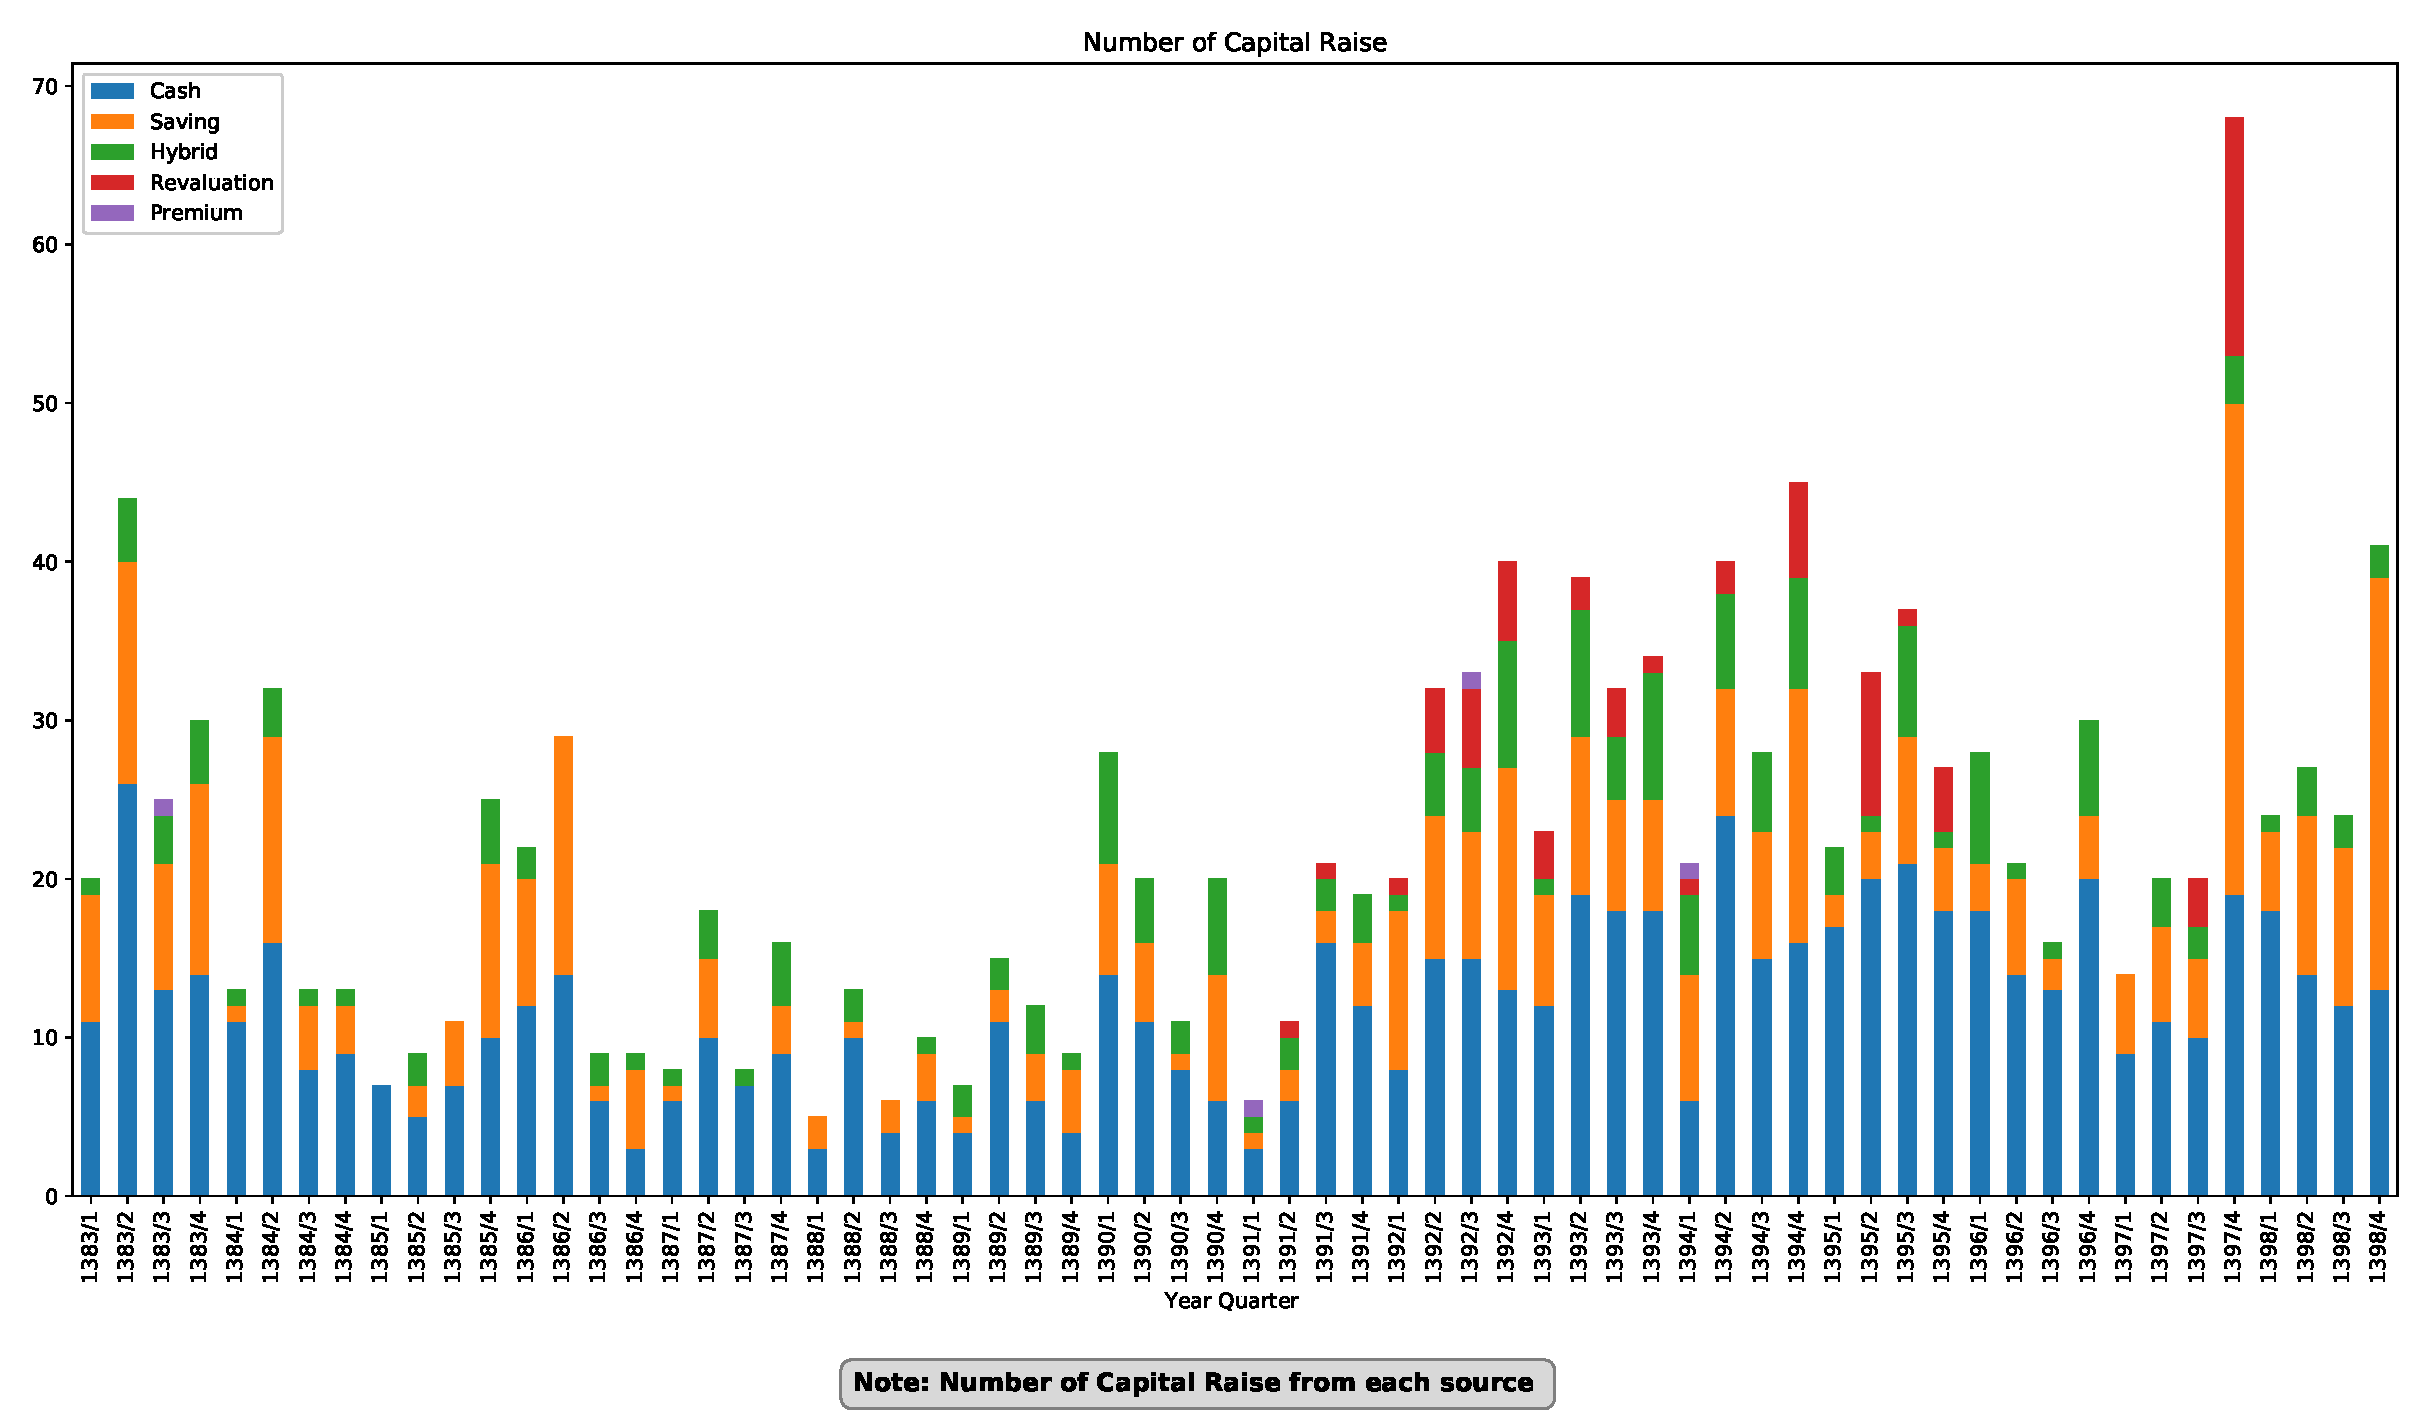
\includegraphics[width=1\linewidth]{Q2Number2}
\caption{}
\label{fig:q2number2}
\end{figure}
\end{landscape}





\begin{figure}
\centering
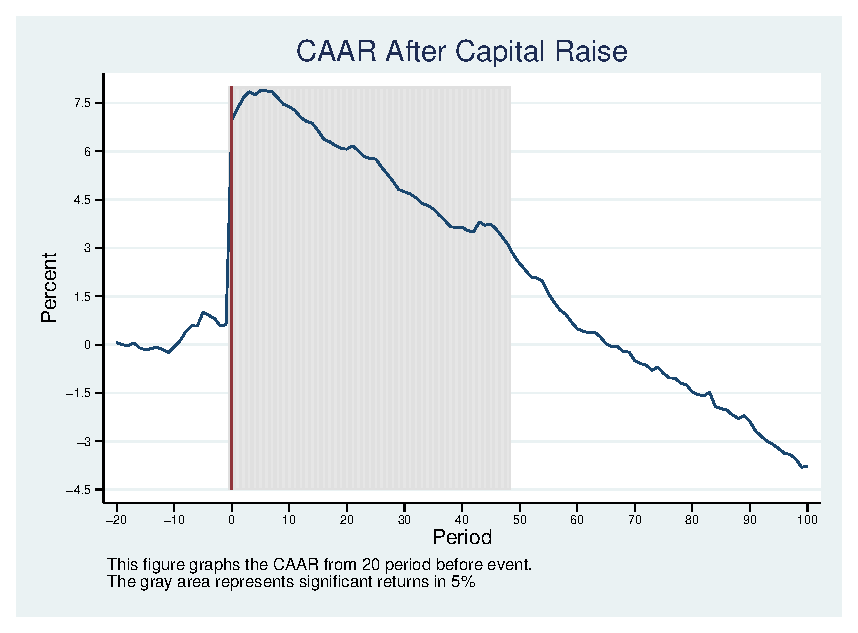
\includegraphics[width=0.7\linewidth]{AbReturn.eps}
\caption{}
\label{fig:abreturn}
\end{figure}

\begin{figure}
\centering
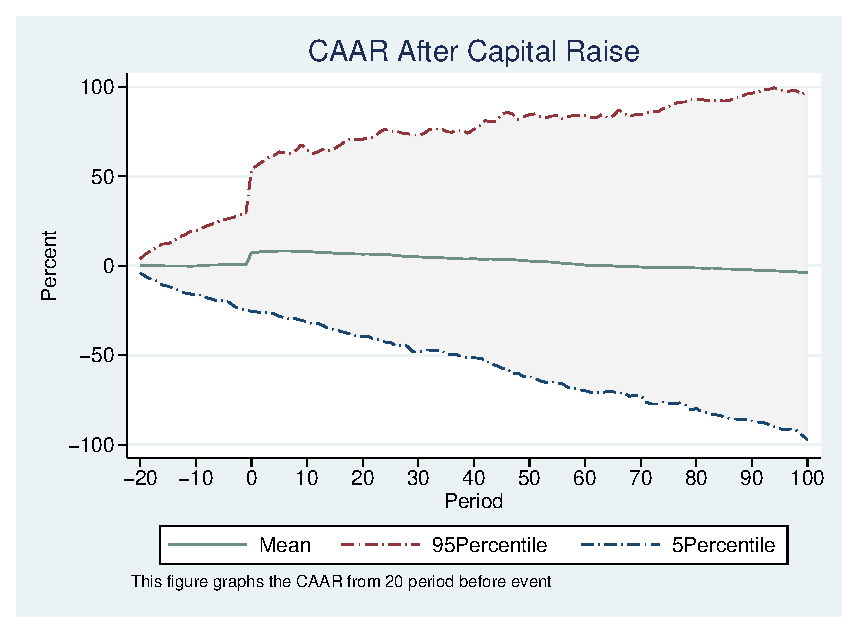
\includegraphics[width=0.7\linewidth]{95-5AbReturn.eps}
\caption{}
\label{fig:955abreturn}
\end{figure}




\begin{figure}
\centering
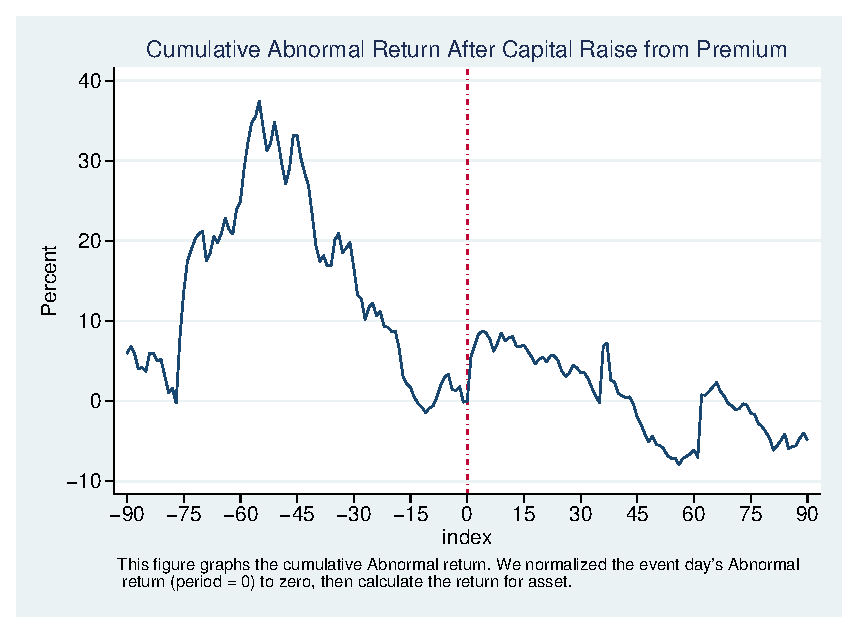
\includegraphics[width=0.7\linewidth]{AbReturnPremium}
\caption{}
\label{fig:abreturnpremium}
\end{figure}
\begin{figure}
\centering
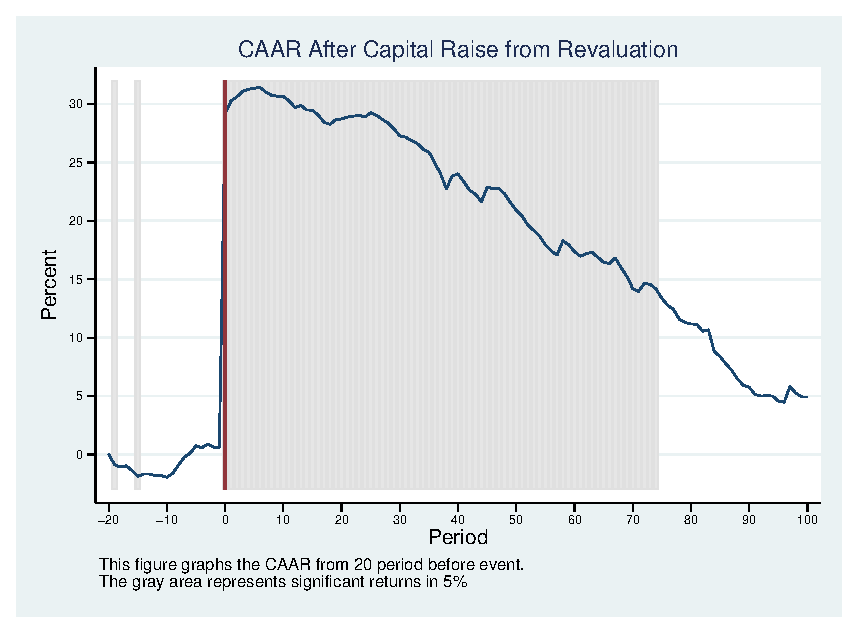
\includegraphics[width=0.7\linewidth]{AbReturnRevalution}
\caption{}
\label{fig:abreturnrevalution}
\end{figure}
\begin{figure}
\centering
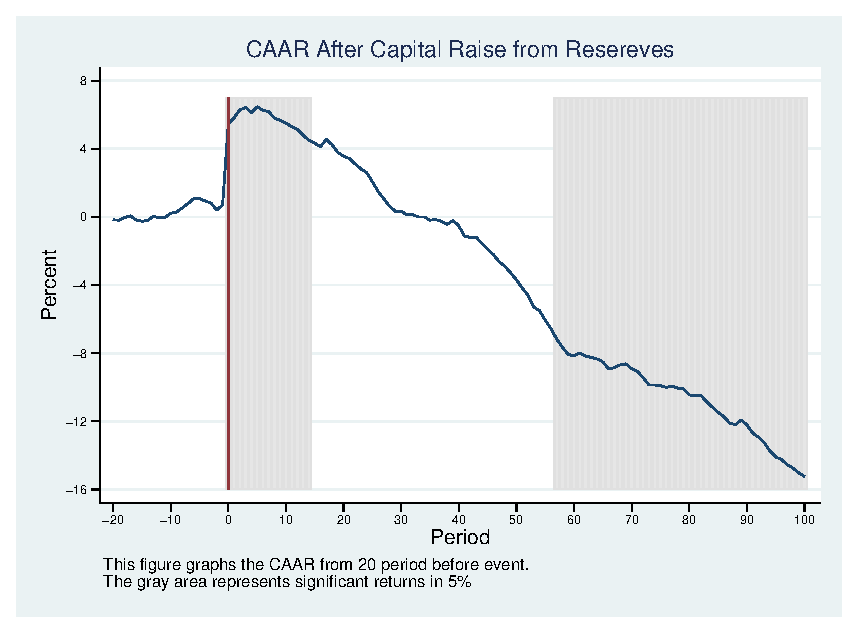
\includegraphics[width=0.7\linewidth]{AbReturnSaving}
\caption{}
\label{fig:abreturnsaving}
\end{figure}
\begin{figure}
\centering
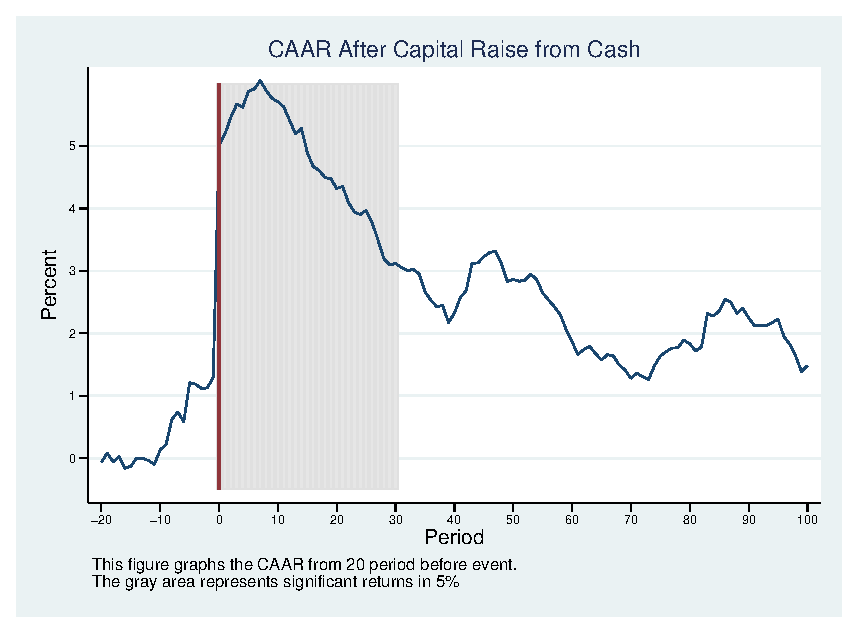
\includegraphics[width=0.7\linewidth]{AbReturnCash}
\caption{}
\label{fig:abreturncash}
\end{figure}
\begin{figure}
\centering
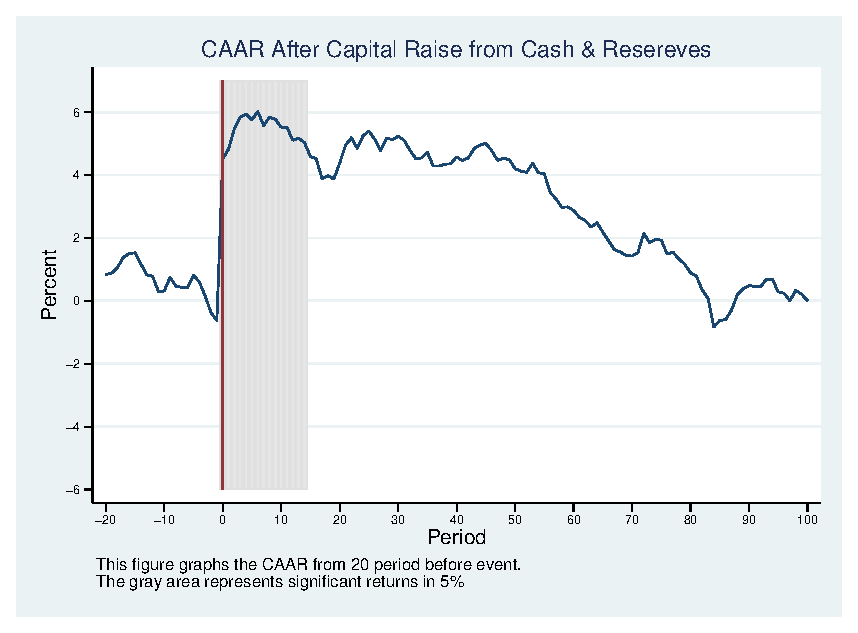
\includegraphics[width=0.7\linewidth]{AbReturnHybrid}
\caption{}
\label{fig:abreturnhybrid}
\end{figure}




\begin{figure}
\centering
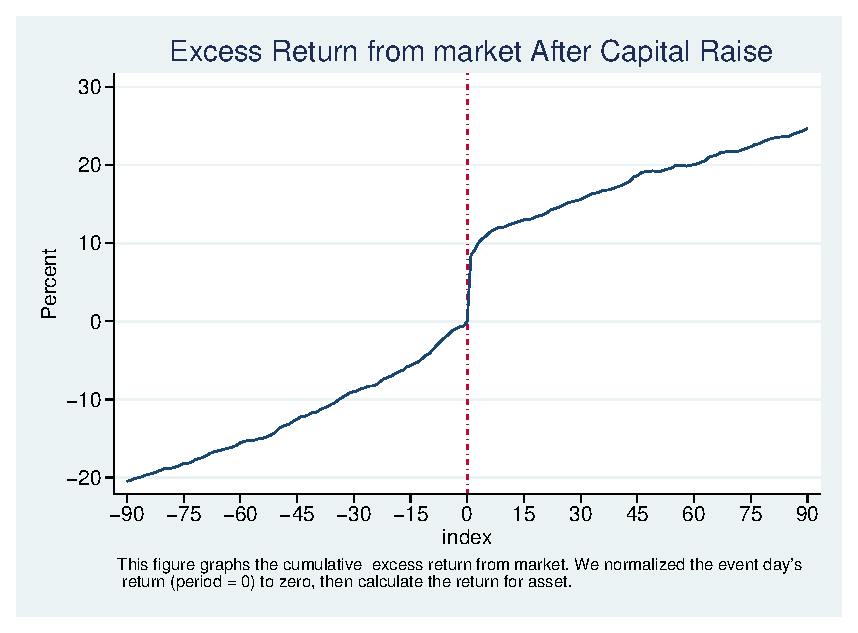
\includegraphics[width=0.7\linewidth]{EReturn}
\caption{}
\label{fig:ereturn}
\end{figure}

\begin{figure}
\centering
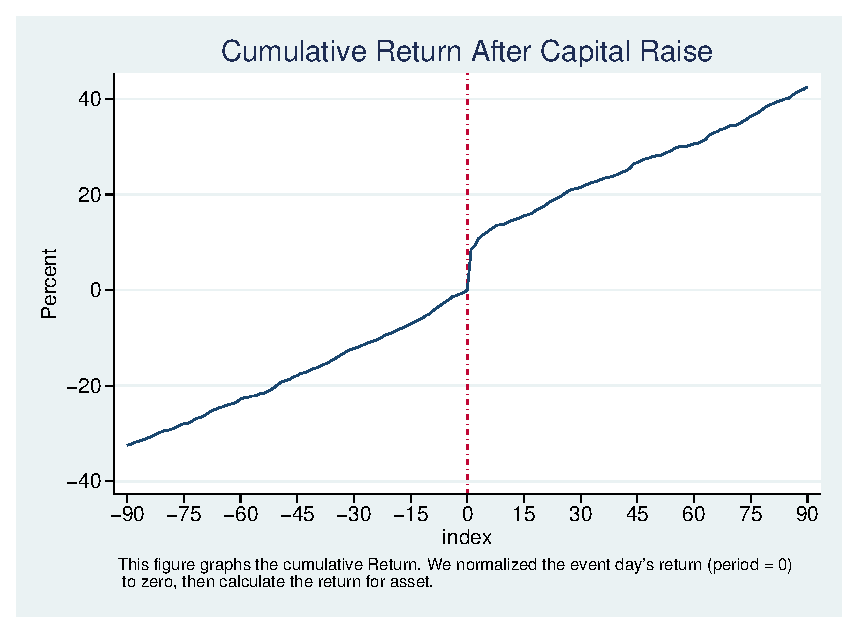
\includegraphics[width=0.7\linewidth]{Return}
\caption{}
\label{fig:return}
\end{figure}



\end{document}